\subsection{La confidentialité différentielle}
%ajouter du texte sur la confidentialité confidentielle
La confidentialité différentielle est l'une des techniques les plus populaires ces dernières années surtout dans la recherche. En effet, contrairement aux autres techniques, elle est la seule à pouvoir fournir des preuves mathématiques sur la possibilité de borner l'information qui peut être apprises sur un individu.

\subsubsection{Formalisation}
soit \begin{math}\epsilon\end{math} un réel et\begin{math}A\end{math} une algorithme probabiliste qui prend pour entrée un jeu de données. Soit \begin{math}imgA\end{math} image de \begin{math}A\end{math}. L'algorithme \begin{math}A\end{math} et dit \begin{math}\epsilon\end{math}-différentiellement confidentiel, si, pour tous jeux de données \begin{math}D_{1}\end{math} et \begin{math}D_{2}\end{math} qui différèrent d'une seul élément(l'information à propos d'une seule personne) et pour sous ensemble \begin{math}S\end{math} de \begin{math}imgA\end{math},

\[
Pr[A(D_{1})\in S] \leq e^{\epsilon} * Pr[A(D_{2})\in S]
\]
où la probabilité est fondée sur l'aléa introduit par l'algorithme. D'après cette définition, la confidentialité différentielle porte sur l'algorithme lui-même, et non sur les données traitées.
\subsubsection{Exemple}
Soit une base de données médicale \begin{math}D_{1}\end{math}, dans laquelle chaque enregistrement contient deux informations \textbf{(Nom,X)} où X est un booléen qui indique si une personne a le diabète ou non.
\begin{figure}[!h]
    \centering
    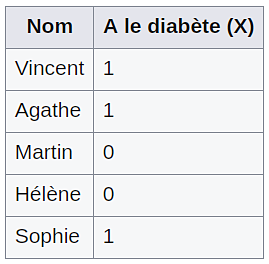
\includegraphics[width=.3\textwidth]{images/anonymisation/confidentialite_diff.png}
    \caption{ exemple confidentialité différentielle}
    \label{fig:exemple confidentialité différentiellel}
\end{figure}
On suppose qu'un utilisateur malintentionné veut connaître l'état de santé de Sophie. On suppose également qu'il connaît ligne qui correspond à Sophie(Ligne 5). L'utilisateur n'est autorisé à questionner la base qu'à travers d'une Fonction \begin{math}F_{i}\end{math} qui renvoie une somme des \begin{math}i\end{math} premières lignes. Cet utilisateur peut connaître l'état de santé de Sophie en faisant un simple Différence entre \begin{math}F_{5}(D_{1}) = 3\end{math} et \begin{math}F_{4}(D_{1}) = 2\end{math}

En poursuivant avec cet exemple, si l'on construit maintenant une base D2 en remplaçant(Sophie,1) par (Sophie, 0) alors cet utilisateur sera capable de ditinguer \begin{math}D2\end{math} et \begin{math}D1\end{math} en calculant la différence \begin{math}F_{5} - F_{4}\end{math}. S'il était amené à recevoir les valeurs \begin{math}F_{i}\end{math} via un algorithme \begin{math}\epsilon\end{math}-différentiellement confidentiel, pour un \begin{math}\epsilon\end{math} suffisamment petit, alors il serait incapable de faire la différence entre \begin{math}D_{2}\end{math} et \begin{math}D_{1}\end{math}.

\paragraph{Évaluation de la confidentialité différentielle}
\begin{itemize}
    \item \textbf{Individualisation:} si les résultats se limitent à la production de statistiques et si les règles appliquées à l’ensemble de données sont bien choisies, il ne devrait pas être possible d’utiliser les réponses pour isoler un individu. 

    \item \textbf{Corrélation:} en recourant à des requêtes multiples, il pourrait être possible de relier entre elles les entrées relatives à un individu spécifique d’une réponse à l’autre. 

    \item \textbf{Inférence:} il est possible de déduire des informations concernant des individus ou des groupes au moyen de requêtes multiples. 
\end{itemize}